\documentclass{IEEEtran}
\usepackage{graphicx}
\usepackage{amsmath}
\usepackage{cite}
\usepackage{booktabs}
\usepackage{caption}
\usepackage{amsfonts}
\usepackage{listings}
\usepackage{array}
\usepackage{listings}
\newcolumntype{P}[1]{>{\centering\arraybackslash}p{#1}}
\DeclareCaptionType{equ}[][]


\markboth{Kernels methods for machine learning : Class 2022-2023, MVA MSc}{Last Name \MakeLowercase{\textit{et al.}}: Title}

\title{
    \huge{
        Report on the Kaggle Data Project
        for
        MVA 22-23 Kernels Methods Class.
        }
}
\author{Louis BLAZEJCZAK-BOULEGUE, Romain SÉAILLES\\
Kernels Methods for Machine Learning Class 2022-2023, MVA MSc\\
    \{louis.blazejczak-boulegue, romain.seailles\}@etu.minesparis.psl.eu
}
\begin{document}
\maketitle

\section{The Challenge}

The goal of this challenge was to process molecules represented as graphs and predict their activity based on their structure. The key requirement for the challenge was to accomplish this task using kernel methods only. This challenge took place in our MVA class, and it presented an opportunity to learn how to implement machine learning algorithms using kernel methods.

The available data were a training dataset composed of 6000 annotated molecules used for training and 1000 non-annotated molecules for testing purposes. Teams were required to submit their predictions for the test set to Kaggle for evaluation.

\section{Pipeline}

\subsection{Structure}
We choose to develop using Python and C++ mainly.

Our project's structure looks like this:

\begin{figure}[h]
    \begin{lstlisting}[frame=none,basicstyle=\ttfamily]
        project/
        |-- data/
        |-- export/
        |-- kernels/
        |-- rapport/
        |-- results/
        |-- biblio/
        |-- dataset/
        |-- optimization/
        |-- run.py
        |-- treeEditDistance/
        |-- configs/
        |-- env/
        |-- preprocessing/
        |-- requirements.txt
        `-- svc/
    \end{lstlisting}
    \captionof{figure}{Project Structure}
    \label{fig:project-structure}
\end{figure}


Here is the converted LaTeX item list:

\begin{itemize}
    \item \texttt{data/}: This folder contains test and training datasets and labels.
    \item \texttt{export/}: This folder contains the resulting \texttt{.csv} file after running kernels that can be submitted in Kaggle.
    \item \texttt{kernels/}: This is where all the kernel code is located. It contains the main class kernel, as well as every subclass implementing a different kernel.
    \item \texttt{rapport/}: This folder contains the Latex file used to produce this article.
    \item \texttt{results/}: This folder contains all the results tables for each run. This allows us to compare the performance of kernels among each other.
    \item \texttt{biblio/}: This folder contains the resources we read.
    \item \texttt{dataset/}: This folder includes dataset classes that implement cross-validation.
    \item \texttt{optimization/}: This folder contains the framework to tune the hyperparameters of our kernel using a Bayesian search algorithm.
    \item \texttt{run.py}: This is the main entry point of our program. It can evaluate the performance of a given kernel and produce predictions on the test dataset.
    \item \texttt{treeEditDistance/}: This is a Python module written in C++ useful to compute the GWWL kernel, which will be detailed later on.
    \item \texttt{configs/}: This folder contains all the configured kernels. A unique kernel can be deployed using multiple config files with different parameters. For instance, there is only one WL kernel, but there are multiple WL config files that deploy this kernel with different depths. Those config files are given to \texttt{run.py} to be tested.
    \item \texttt{env/}: This folder contains our Python environment.
    \item \texttt{preprocessing/}: This folder includes useful functions such as \texttt{load\_data}, for example.
    \item \texttt{requirements.txt}: This file lists all our Python dependencies.
    \item \texttt{svc/}: This folder implements our custom SVC implementation.
\end{itemize}

Note that we deployed several \texttt{unittest}s to test important objects, especially SVC and kernels. These were tested against the well-known scikit-learn implementation. This protocol ensures that any modification, especially towards optimization, will not break our work pipeline. Furthermore, it ensures that our tools are accurate and that our results are reproducible.

\subsection{Comparing different solutions}
We performed cross-validation to compare the effectiveness of different kernels. We chose to use a 6-fold cross-validation process on the molecule dataset, which consisted of 6000 molecules. The dataset was randomly split into six sets of 1000 molecules each, with a fixed seed for reproducibility.

For each fold in the cross-validation process, one set was separated for testing while the other five were used for training. This means that each fold involved training a Support Vector Classifier (SVC) on 83\% of the data and testing it on the remaining 17\%.

Given the heaviness of the class imbalance in our dataset, we opted to use the F1 score as our primary evaluation metric. We also measured accuracy, precision, and recall for informational purposes. However, we mainly relied on the ROCAUC to evaluate the performance of our project.

Table [REF] shows the results of our tests for one kernel.
Similar output tables for all tested kernels are store in the \texttt{results/} directory.

\begin{table}[h]
    \centering
    \begin{tabular}{l||llll|l}
                & Accuracy & Precision & Recall & F1     & ROCAUC \\
        \hline \hline
        Fold 1  & 93.0\%   & 52.2\%    & 64.9\% & 57.8\% & 88.2\% \\
        Fold 2  & 88.3\%   & 47.3\%    & 74.1\% & 57.8\% & 89.4\% \\
        Fold 3  & 88.2\%   & 40.0\%    & 77.6\% & 52.8\% & 89.5\% \\
        Fold 4  & 92.1\%   & 65.9\%    & 54.2\% & 59.5\% & 88.0\% \\
        Fold 5  & 93.1\%   & 64.0\%    & 53.3\% & 58.2\% & 87.9\% \\
        Fold 6  & 93.0\%   & 61.3\%    & 62.6\% & 62.0\% & 90.8\% \\
        \hline
        Average & 91.3\%   & 55.1\%    & 64.5\% & 58.0\% & 89.0\% \\
    \end{tabular}
    \caption{Example of the output table for one of the tested kernels, \emph{WL-depth4}.}
    \label{tab:example}
\end{table}

Please refer to the online Github repository for further details [REF]. Additionally, all our results are available in the appendix.
https://github.com/RSLLES/KernelMethodsDataChallenge/blob/main/results/README.md

\subsection{Optimizing a solution}
To optimize our chosen kernel parameters, we used the same 6-fold cross-validation method as previously mentioned. However, in this step, we performed a Bayesian search within a parameter grid to obtain optimal values.

This method is highly efficient in fine-tuning parameters because it can optimize functions that are computationally expensive and where gradient computation is not possible. All the results that we present in this report correspond to the best version of a kernel obtained after hyperparameter tuning.



\subsection{Faster Inference}
As we will soon discuss, computing kernels with graphs can be quite expensive. Therefore, it was mandatory to optimize our code as much as possible to avoid any loss of time and ensure optimal overall performance.

Firstly, the kernel's gram matrix was computed and then split according to specific indices for each fold. This strategy prevents extensive recomputation. When fitting the SVC (i.e., computing the support vectors given the training set), only half of the matrix was computed as the matrix is symmetric positive definite.

Furthermore, nearly all our kernels can be decomposed into two steps: a heavy step computing an embedding form of a graph (similar to the embedding $\phi(x)$ in the RKHS) and a lighter operation between those two embeddings (similar to the inner product in the RKHS). Given the pipeline before, with one graph (resp two) of size $n$ (resp $n,m$), one can see that the heavy method phi could only be called $n$ (resp $n+m$) times at the beginning, while the lighter operation must be called to fill the gram matrix, i.e., $n(n+1)/2$ (resp $n*m$) times. Untangling those operations drastically increases performances as it decreases the program's complexity by one degree.

Finally, we deployed multiprocessing to use as many cores as possible and make the calculation as fast as possible. Special attention was given to using only NumPy's methods as they are compiled in C and thus efficient.

Some kernels (especially GWWL) were still too slow even with these tricks, so we decided to recreate them in C++, which is significantly faster than Python due to its compiled nature. Furthermore, we also moved the outer loop (computing the gram matrix) in the C++ module to benefit from native multithreading and avoid any useless back and forth between Python and our module. Finally, we implemented a common cache system to reduce computation.

\subsection{The Code}
Our complete project is published on GitHub and can be cloned at the following address: ``https://github.com/RSLLES/KernelMethodsDataChallenge''.
\section{SVC}

Louis


\section{Kernels}

The literature on graph kernels is vast and constantly evolving due to active research and development. To begin our work, we reviewed the literature and explored state-of-the-art kernel techniques for the current solution. Considering its recent good performance,
we chose to focus on variants of the Weisfeiler-Lehman kernel.

\subsection{Weisfeiler-Lehman}
As part of our project, we implemented and experimented with the Weisfeiler-Lehman (WL) method, a graph isomorphism algorithm originally designed by Weisfeiler and Lehman in 1968. The algorithm aims to determine if two graphs are isomorphic with one-sided error.

The core idea of the WL method is to repeatedly refine a partition of the vertex set, where each node's label and those of its neighbors are concatenated, sorted, and hashed to produce a new label. The hash function employed by the algorithm should be as perfect as possible, meaning that different sets of labels should never be mapped to the same new label. With each iteration, larger substructures are incorporated into the labels, allowing the algorithm to capture more complex patterns in the graph. Finally, the new graphs after each iteration can be compared using a relatively simple algorithm, as the deeper the algorithm goes, the more information is encapsulated from the neighborhood of every node.
The following figure - extracted from the original paper - details the process.

Figure \ref{fig:wlmethod} - extracted from the original paper - details the process.

\begin{figure}[h]
    \centering
    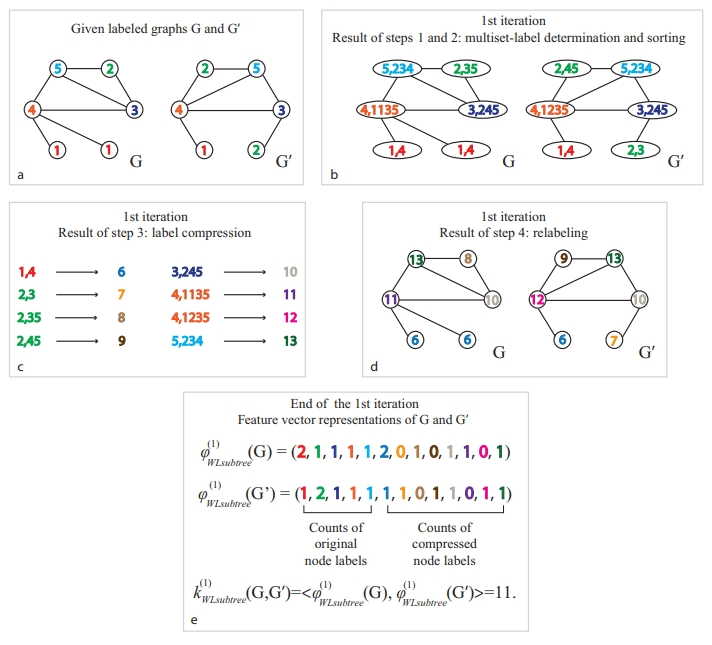
\includegraphics[width=\linewidth]{wl_process.jpg}
    \caption{The WL Method.}
    \label{fig:wlmethod}
\end{figure}

Moreover, this kernel is exceptionally computationally efficient. Indeed, all the embeddings can be computed separately for each node, and the final comparison is also quite simple, resulting in an overall high efficiency.

A fast and straightforward approach to compare graphs would be to evaluate the frequency of their nodes.
For each subgraph iteratively computed during the WL process,
all of its nodes can be compared with all the nodes of another graph,
using a Kronicker metric.
More formally, given two graphs $G_1$ and $G_2$
with respective nodes $\mathcal{N}_1$, $\mathcal{N}_2$, let $l(n)$
be the label associated with the node $n$ in either $\mathcal{N}_1$ or $\mathcal{N}_2$.
Then the kernel can be formulated as:

\begin{equation*}
    K(G_1, G_2) = \sum_{n_1 \in \mathcal{N}_1} \sum_{n_2 \in \mathcal{N}_2} [1 - \delta_{l(n_1), l(n_2)}]
\end{equation*}
where $\delta_{l(n_1), l(n_2)} = 1$ \text{ if } $l(n_1) = l(n_2)$ and $0$ otherwise.

This approach is known as the Weisfeiler-Lehman Subtree Kernel, and it has been widely studied in the literature.
We proove that this kernel is positive semi-definite.
First, note that every label is an integer,
as we use a hash function from $\mathbb N $ to $\mathbb N $.
We embed a node $n$ with a sequence $u^{(n)}$ such that
$\forall k \in \mathbb{N}, u^{(n)}k = 1$ if $k = l(n)$, 0 otherwise.
As each node has a unique label, $\sum{k=0}^\infty u^{(n)}_k = 1$,
hence it is absolutely convergent, and thus, the following scalar product is well-defined over the space of absolute convergent sequences:

\begin{equation*}
    \forall u^{(n_1)}, u^{(n_2)}, < u^{(n_1)} \; | \; u^{(n_2)} > =
    \sum_{k=0}^\infty u^{(n_2)}_k u^{(n_1)}_k
\end{equation*}

Therefore, the kernel is positive definite.

Given a sequence of graphs $G^{(k)}$ obtained after the $k$-iteration of the WL process,
one can simply sum the results of the kernel described above at each level, creating a positive definite kernel.

After optimization, we found that this kernel achieves its best performances using a depth of $4$:

\begin{table}[h]
    \centering
    \begin{tabular}{l|llll|l}
                & Accuracy & Precision & Recall & F1     & ROCAUC \\
        \hline
        Average & 91.3\%   & 55.1\%    & 64.5\% & 58.0\% & 89.0\% \\
    \end{tabular}
    \caption{\emph{WL-depth4} performances.}
    \label{tab:wldepth4}
\end{table}

The code for this kernel is available in our repository : \texttt{kernel/WL.py}.

\subsection{WL-edges}
The previous model did not take into account the labels associated with edges. To address this issue, we chose to include the label of the edge in the label of a node's neighborhood when constructing its new label in the WL scheme.

Previously, given a node $n$ in a graph $G$, when considering one of its neighbors $n'$, we used $l(n')$ as the label for $n'$. However, we now consider $\operatorname*{hash}(l(n'), l(\operatorname{edge}(n, n')))$, which combines the labels of the node and the edge that connects them.

We found that this simple modification led to a significant improvement in retrieval performance.
As shown in Table \ref{tab:wldepth6edge}, the average accuracy, precision, recall, F1-score, and ROCAUC increased when we applied this modification.


\begin{table}[h]
    \centering
    \begin{tabular}{l|llll|l}
                & Accuracy & Precision & Recall & F1     & ROCAUC \\
        \hline
        Average & 93.0\%   & 64.0\%    & 55.1\% & 59.2\% & 90.3\% \\
    \end{tabular}
    \caption{\emph{WL-edge-depth6} performances.}
    \label{tab:wldepth6edge}
\end{table}

From our experiments with various kernels, we observed that adding the edge label information in the WL process consistently led to better performance. Therefore, all of the following kernels include this modification, even if it is not specified explicitly.

The code for this kernel is available in our repository : \texttt{kernel/WL.py}
with \texttt{edges\_labels = True}.

\subsection{WL variants}
Since the Weisfeiler-Lehman Subtree Kernel is based on a relatively simple update scheme,
we believe that there is potential for improvements in this area.

To begin with, we note that the previous version of the Weisfeiler-Lehman Subtree Kernel can be reformulated
as a Vertex Histogram Kernel. Indeed,
given a graph $G$, we denote by $m_G(l(n))$ the multiplicity of
the label $l(n)$ in the graph $G$ (with $m_G(l(n)) = 0$ if $n$ is not an
element of $\mathcal N_G$). Denoting by $L_G = \{l(n), n \in \mathcal N_G\}$
the set containing all the labels of the nodes in $G$,
one can easily check that these two formulations are equivalent:
\begin{equation*}
    \begin{split}
        K(G_1, G_2) & = \sum_{n_1 \in \mathcal{N}_1} \sum_{n_2 \in \mathcal{N}_2} [1 - \delta_{l(n_1), l(n_2)}]\\
        &= \sum_{l \in L_{G_1} \cup L_{G_2}} m_{G_1}(l)m_{G_2}(l)
    \end{split}
\end{equation*}

Therefore, we tried slightly varying this kernel, based on the kernel presented in class as an exercise:

\begin{itemize}
    \item The Minimum Vertex Histogram Kernel

          \begin{equation*}
              K(G_1, G_2) = \sum_{l \in L_{G_1} \cup L_{G_2}} \operatorname*{min}(m_{G_1}(l), m_{G_2}(l))
          \end{equation*}

    \item The Min over Max Vertex Histogram Kernel
          \begin{equation*}
              K(G_1, G_2) = \sum_{l \in L_{G_1} \cup L_{G_2}} \frac{\operatorname*{min}(m_{G_1}(l), m_{G_2}(l))}{\operatorname*{max}(m_{G_1}(l), m_{G_2}(l))}
          \end{equation*}
    \item The Arithmetic Vertex Histogram Kernel
          \begin{equation*}
              K(G_1, G_2) = \sum_{l \in L_{G_1} \cup L_{G_2}} \frac{\operatorname*{GCD}(m_{G_1}(l), m_{G_2}(l))}{\operatorname*{LCM}(m_{G_1}(l), m_{G_2}(l))}
          \end{equation*}
\end{itemize}

Overall, these slight variants performed below our last baseline \emph{WL-edges-depth6}.
Results can be found in Table \ref{tab:method_comparison_depth4}.
\begin{table}[h]
    \centering
    \begin{tabular}{l|llll|l}
        Method    & Accuracy & Precision & Recall & F1     & ROCAUC \\
        \hline
        min-WL    & 93.2\%   & 64.9\%    & 57.8\% & 61\%   & 89.7\% \\
        minmax-WL & 93.3\%   & 67.1\%    & 54\%   & 59.8\% & 89.3\% \\
        arithm-WL & 93.4\%   & 67.7\%    & 54.3\% & 60.3\% & 88.5\% \\
    \end{tabular}
    \caption{Performances of Min-WL, MinMax-WL and Arithm-WL at depth 4 with edges.}
    \label{tab:method_comparison_depth4}
\end{table}

The code for those kernels is available in our repository : \texttt{kernel/WL.py}.

\subsection{Jensen-Shannon Weisfeiler-Lehman Kernel}

During our search for new kernels to try, we realized that the Vertex Histogram Kernel formulations (which refer to the frequency of each label inside a given graph) could be interpreted as a probability measure simply by normalizing.
Formally, given a graph $G$, we could extract a probabilty measure
$\rho$ such that :

\begin{equation*}
    \forall l \in \mathbb N, \rho (l) = \frac{m_G(l)}{\sum_{\lambda \in L_G}{m_G(\lambda)}}
\end{equation*}

We were now facing the question of comparing two probability measures. The first idea that came into our mind was to use Kullback-Leibler divergence. Unfortunately, this divergence is not symmetric and therefore cannot be used as a kernel. During our research, however, we found the Jensen-Shannon divergence. It is a smooth and symmetric version of the Kullback-Leibler divergence.

Given two probabilty distribution $P$ and $Q$, we denote their
Jensen-Shannon divergence as :

\begin{equation*}
    JS(P, Q) = \frac{1}{2}KL(P|M) + \frac{1}{2}KL(Q|M)
\end{equation*}
where $M = \frac{1}{2} \left( Q + P \right)$ and $KL$ is the Kullback-Leibler divergence.

After some searching, we found that the Jensen-Shannon divergence is a conditional negative function \cite{callut2011sequence}.
Therefore, according to a theorem we found in \cite{callut2011sequence},
given a conditional negative function $ f : \mathcal{X} \times \mathcal{X} \to R$,
the kernel $K : \mathcal{X} \times \mathcal{X} \to R$ defined such that:
$\forall x, y \in \mathcal{X}, K(x, y) = \exp{(- \lambda f(x,y))}$
is positive definite with $\lambda > 0$.

Furthermore, a nice property of this kernel is
that the Jensen-Shannon divergence can be rewritten using the
the Shannon entropy, denoted $H$. It can be shown that:

\begin{equation*}
    JS(P, Q) = H(M) - \frac{1}{2} \left( H(Q) + H(P) \right)
\end{equation*}
The attentive reader might notice that
$H(P)$ and $H(Q)$ can be precomputed ahead of time,
leading to a very fast implementation.

The results using this kernel are shown in Table \ref{tab:jswl}. This kernel proves to be quite performant, achieving new best results during our project. Furthermore, it involved very low computation resources, making it by far the fastest kernel to achieve such good results.

We found relatively few references surrounding this kernel, and we believe that it may be a good subject for further research since such a naive implementation gives great results.
\begin{table}[h]
    \centering
    \begin{tabular}{l|llll|l}
                & Accuracy & Precision & Recall & F1     & ROCAUC \\
        \hline
        Average & 93.6\%   & 84.1\%    & 37.4\% & 51.7\% & 91.6\% \\
    \end{tabular}
    \caption{\emph{JSWL-edges-depth3} performances.}
    \label{tab:jswl}
\end{table}

The code for this kernel is available in our repository : \texttt{kernel/JSWL.py}.

\subsection{Wasserstein Weisfeiler-Lehman Kernels}

The recent paper \cite{togninalli2019wasserstein}
caught our attention by it's impressive performance
on multiples up to date reviews.

caught our attention due to its impressive performance on multiple up-to-date reviews. The authors propose using the classic Weisfeiler-Lehman process to compute the similarity between two nodes. For a node $n$, one can compute a sequence of labels using the Weisfeiler-Lehman scheme:
$$\begin{pmatrix} l^{(0)}(n) & l^{(1)}(n) & \dots & l^{(d)}(n)\end{pmatrix} $$
where $d$ is the final depth of the process.

Using this representation, one can create a metric that compares the similarity of two nodes as follows:
\begin{equation*}
    \forall n_1 \in \mathcal{N}_1, n_2 \in \mathcal{N}_1,
    d_{n_1, n_2} = \frac{1}{d} \sum_{s = 0}^d [1 - \delta_{l^{(s)}(n_1), l^{(s)}(n_2)}]
\end{equation*}
where again $\delta_{x, y} = 1$ \text{ if } $x=y$ and $0$ otherwise.

This scheme is similar to the Weisfeiler-Lehman Subtree Kernel. However, instead of summing everything, we kept apart the similarity of each node from $G_1$ vs each node of $G_2$.

Using this process, one can create a matrix $D$ of shape
$(\# \mathcal{N}_1, \# \mathcal{N}_2)$
where $[D]_{i,j}$stores the distance in the sense given above between a node from $G_1$ and a node from $G_2$. Note that the coefficients in $D$ belong to the interval $[0,1]$.

Finally, this matrix can be considered as a distance matrix related to the optimal transport problem. Therefore, a natural metric to consider is the Wasserstein distance, which uses the matrix as input distance between two uniform histograms. As a quick reminder, the Wasserstein distance can be computed by solving an LP program:

\begin{equation*}
    w = \underset{P \in \Gamma}{\operatorname*{min}} \left< P \; | \; D \right>
\end{equation*}

Here, $P$ is a joint matrix containing fractions that indicate how to transport the values from the first event to the second with minimal total transport effort. Finally, the authors proved that the kernel $K(G_1,G_2) = \exp(-\lambda w)$ is positive definite.

This theory links the optimal transport theory with graph similarity, a process we found quite original and interesting. Furthermore, many sources acknowledge the performance of this kernel, and it is becoming a new stepping stone in the graph kernel world.

The code for this kernel is available in our repository : \texttt{kernel/WWL.py}.
We used an external library to compute the Wasserstein distance.
However, the reader may keep in mind that this kernel is more
computationally expensive than all the previous one.

Table \ref{tab:wwl} presents the results we obtained using this kernel, which achieved our best performance on both Kaggle and our local validation test.

\begin{table}[h]
    \centering
    \begin{tabular}{l|llll|l}
                & Accuracy & Precision & Recall & F1     & ROCAUC \\
        \hline
        Average & 93.9\%   & 87\%      & 39.8\% & 54.5\% & 91.8\% \\
    \end{tabular}
    \caption{\emph{WWL-edges-depth3} performances.}
    \label{tab:wwl}
\end{table}

\subsection{Generalized Wasserstein Weisfeiler-Lehman Kernels}
Finally, the last kernel we work on came from an idea presented by
\cite{schulz2022generalized}.
It relies on the observation that the Weisfeiler-Lehman
did not present any nuance while distinguishing labels.
If two nodes have a different label, then they are treated as different,
regardless of any similarity they might have.
While this is a desired property when constructing an
isomorphic test (which is the oringal purpose of the Weisfeiler-Lehman process),
they arguee that it is not adapted for building a kernel, which should try to grasp
the degree of difference between two instances.

Therefore, the authors



\section{Results and discussions}
\subsection{Individual results}
\subsection{Online results}
\subsection{On the correlation between all kernels}
\subsection{On the relative importance of metrics}

\bibliographystyle{plain}
\bibliography{references}

\end{document}
